\section{Model\-Car  Class Reference}
\label{classModelCar}\index{ModelCar@{Model\-Car}}
The same model as {\bf Model2DRigid\-Car} {\rm (p.\,\pageref{classModel2DRigidCar})}. 


{\tt \#include $<$modelcar.h$>$}

Inheritance diagram for Model\-Car::\begin{figure}[H]
\begin{center}
\leavevmode
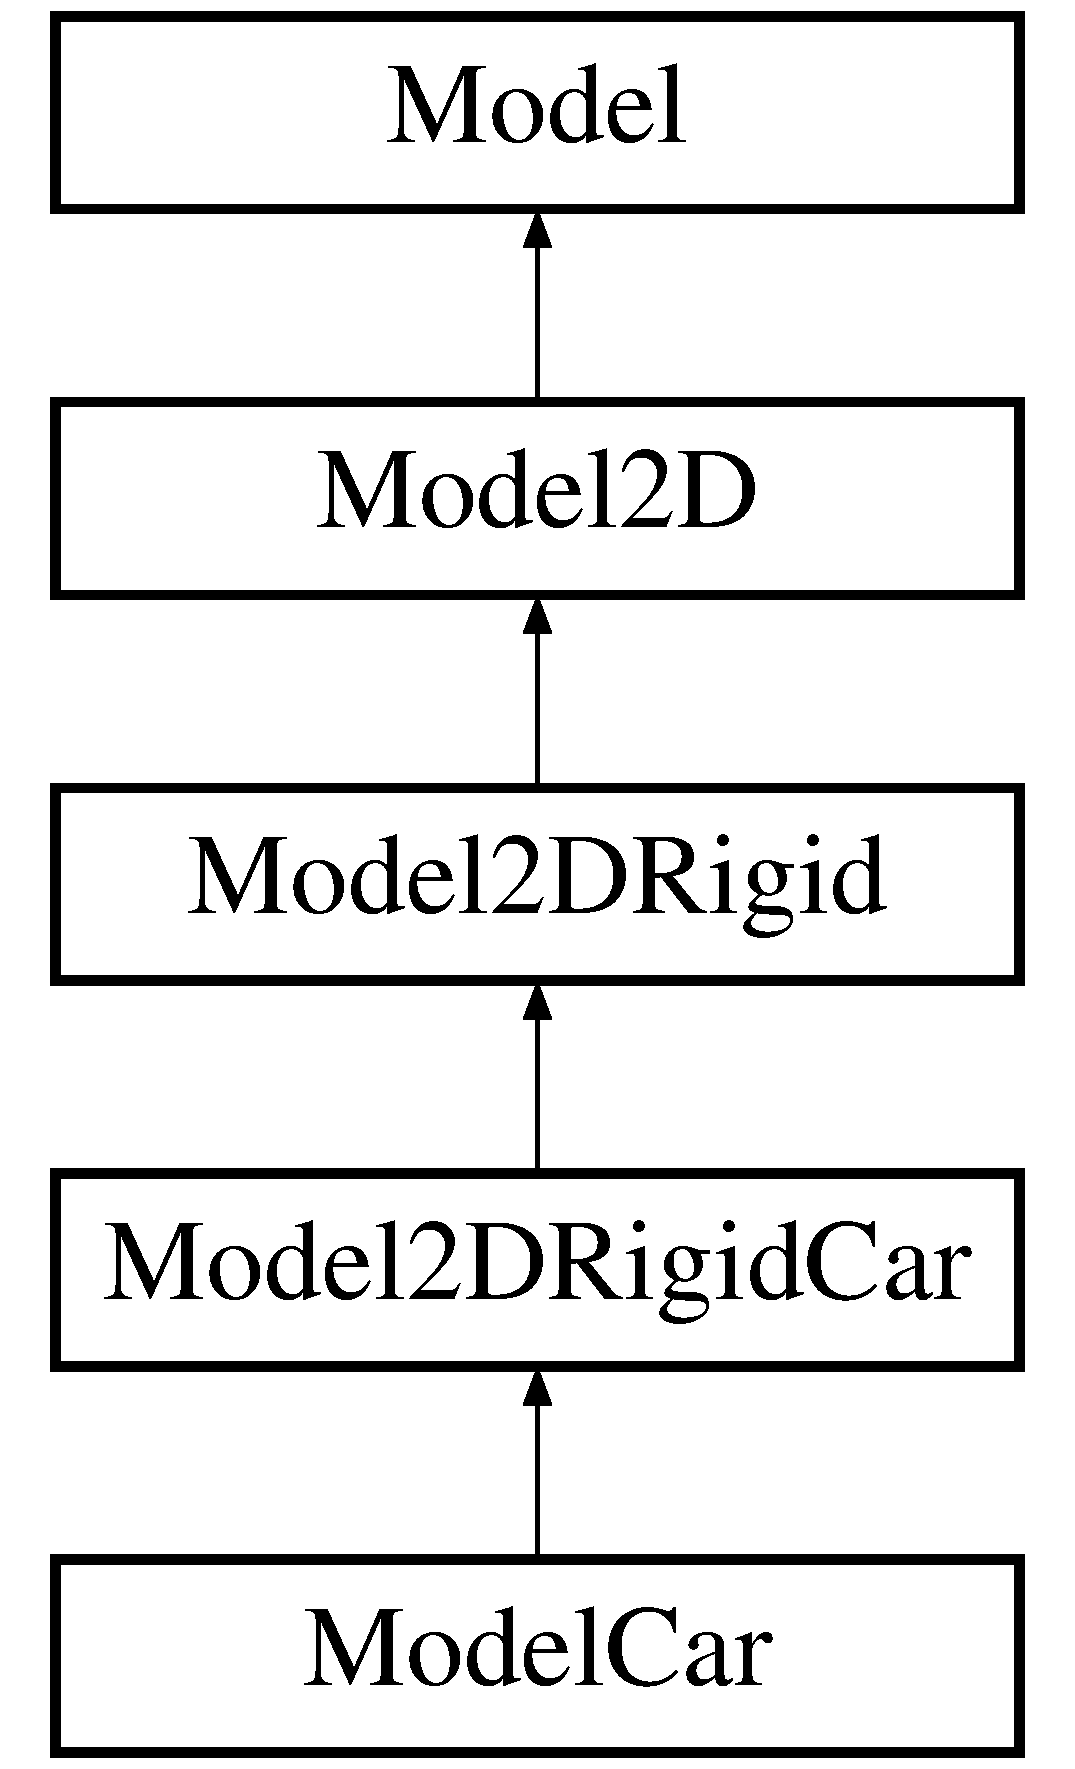
\includegraphics[height=5cm]{classModelCar}
\end{center}
\end{figure}
\subsection*{Public Methods}
\begin{CompactItemize}
\item 
{\bf Model\-Car} (string path)
\item 
virtual {\bf $\sim$Model\-Car} ()
\item 
virtual {\bf MSLVector} {\bf State\-To\-Configuration} (const {\bf MSLVector} \&{\bf x})
\begin{CompactList}\small\item\em A method that converts a {\bf Model} {\rm (p.\,\pageref{classModel})} state in to a {\bf Geom} {\rm (p.\,\pageref{classGeom})} configuration.\item\end{CompactList}\item 
virtual bool {\bf Satisfied} (const {\bf MSLVector} \&state)
\begin{CompactList}\small\item\em Test whether global state-space constraints are satisfied.\item\end{CompactList}\end{CompactItemize}
\subsection*{Public Attributes}
\begin{CompactItemize}
\item 
double {\bf Speed}
\end{CompactItemize}


\subsection{Detailed Description}
The same model as {\bf Model2DRigid\-Car} {\rm (p.\,\pageref{classModel2DRigidCar})}.



\subsection{Constructor \& Destructor Documentation}
\index{ModelCar@{Model\-Car}!ModelCar@{ModelCar}}
\index{ModelCar@{ModelCar}!ModelCar@{Model\-Car}}
\subsubsection{\setlength{\rightskip}{0pt plus 5cm}Model\-Car::Model\-Car (string {\em path})}\label{classModelCar_a0}


\index{ModelCar@{Model\-Car}!~ModelCar@{$\sim$ModelCar}}
\index{~ModelCar@{$\sim$ModelCar}!ModelCar@{Model\-Car}}
\subsubsection{\setlength{\rightskip}{0pt plus 5cm}virtual Model\-Car::$\sim$Model\-Car ()\hspace{0.3cm}{\tt  [inline, virtual]}}\label{classModelCar_a1}




\subsection{Member Function Documentation}
\index{ModelCar@{Model\-Car}!Satisfied@{Satisfied}}
\index{Satisfied@{Satisfied}!ModelCar@{Model\-Car}}
\subsubsection{\setlength{\rightskip}{0pt plus 5cm}bool Model\-Car::Satisfied (const {\bf MSLVector} \& {\em state})\hspace{0.3cm}{\tt  [virtual]}}\label{classModelCar_a3}


Test whether global state-space constraints are satisfied.



Reimplemented from {\bf Model} {\rm (p.\,\pageref{classModel_a4})}.\index{ModelCar@{Model\-Car}!StateToConfiguration@{StateToConfiguration}}
\index{StateToConfiguration@{StateToConfiguration}!ModelCar@{Model\-Car}}
\subsubsection{\setlength{\rightskip}{0pt plus 5cm}{\bf MSLVector} Model\-Car::State\-To\-Configuration (const {\bf MSLVector} \& {\em x})\hspace{0.3cm}{\tt  [virtual]}}\label{classModelCar_a2}


A method that converts a {\bf Model} {\rm (p.\,\pageref{classModel})} state in to a {\bf Geom} {\rm (p.\,\pageref{classGeom})} configuration.



Reimplemented from {\bf Model2DRigid} {\rm (p.\,\pageref{classModel2DRigid_a7})}.

\subsection{Member Data Documentation}
\index{ModelCar@{Model\-Car}!Speed@{Speed}}
\index{Speed@{Speed}!ModelCar@{Model\-Car}}
\subsubsection{\setlength{\rightskip}{0pt plus 5cm}double Model\-Car::Speed}\label{classModelCar_m0}




The documentation for this class was generated from the following files:\begin{CompactItemize}
\item 
{\bf modelcar.h}\item 
{\bf modelcar.C}\end{CompactItemize}
